\documentclass[tikz,border=4pt]{standalone}
\usepackage{amsmath}
\begin{document}
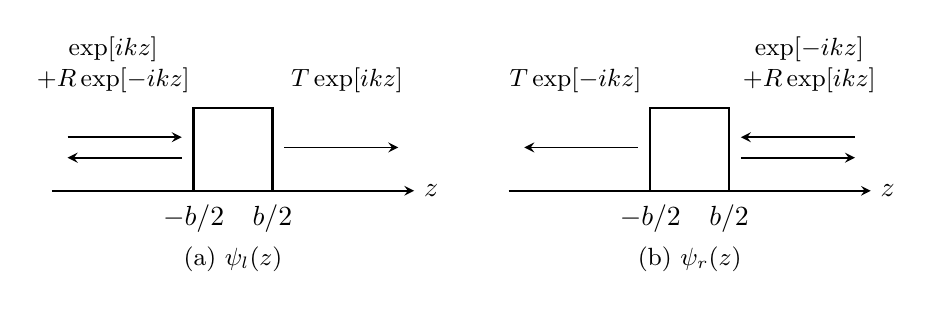
\begin{tikzpicture}[>=stealth, thick, scale=1.0]
  % Left diagram: psi_l (incident from left)
  \begin{scope}[shift={(0,0)}]
    \draw[->, line width=0.55pt] (-2.3, 0) -- (2.3, 0) node[right] {$z$};
    \draw[line width=0.85pt] (-0.5, 0) rectangle (0.5, 1.05);
    \node[below] at (-0.5, -0.05) {$-b/2$};
    \node[below] at (0.5, -0.05) {$b/2$};

    % Incident and reflected arrows on left
    \draw[->, line width=0.6pt] (-2.1, 0.68) -- (-0.65, 0.68);
    \draw[<-, line width=0.6pt] (-2.1, 0.42) -- (-0.65, 0.42);
    % Transmitted arrow on right
    \draw[->, line width=0.6pt] (0.65, 0.55) -- (2.1, 0.55);

    \node[above, align=center, font=\small] at (-1.52, 1.12) {$\exp[ikz]$ \\ $+ R\exp[-ikz]$};
    \node[above, font=\small] at (1.45, 1.12) {$T\exp[ikz]$};
    \node[below, font=\small] at (0, -0.58) {(a) $\psi_l(z)$};
  \end{scope}

  % Right diagram: psi_r (incident from right)
  \begin{scope}[shift={(5.8,0)}]
    \draw[->, line width=0.55pt] (-2.3, 0) -- (2.3, 0) node[right] {$z$};
    \draw[line width=0.85pt] (-0.5, 0) rectangle (0.5, 1.05);
    \node[below] at (-0.5, -0.05) {$-b/2$};
    \node[below] at (0.5, -0.05) {$b/2$};

    % Transmitted arrow on left
    \draw[<-, line width=0.6pt] (-2.1, 0.55) -- (-0.65, 0.55);
    % Incident and reflected arrows on right
    \draw[<-, line width=0.6pt] (0.65, 0.68) -- (2.1, 0.68);
    \draw[->, line width=0.6pt] (0.65, 0.42) -- (2.1, 0.42);

    \node[above, font=\small] at (-1.45, 1.12) {$T\exp[-ikz]$};
    \node[above, align=center, font=\small] at (1.52, 1.12) {$\exp[-ikz]$ \\ $+ R\exp[ikz]$};
    \node[below, font=\small] at (0, -0.58) {(b) $\psi_r(z)$};
  \end{scope}
\end{tikzpicture}
\end{document}
